Nesse ponto, serão apresentados dados da execução da solução apresentada pelo
trabalho.
Algumas imagens serão demonstradas demonstrando o tempo de execução e a memória
utilizada.
Vale ressaltar que os tempos de execução foram computados usando o temporizador
nativo do Python pela biblioteca texttt{time} sendo que o tempo da leitura do
arquivo de entrada foi ignorado.
A obtenção da memória utilizada pelo programa foram obtidos pelo uso do Valgrind.
Além disso as funções que imprimem a saída também foram removidas nas análises.
O comando para executar a solução do trabalho usando o arquivo
\texttt{sarscov2.fasta} é:

\lstset{language=bash}
\begin{lstlisting}[frame=single]
$ python3 main.py sarscov2.fasta
\end{lstlisting}

\begin{figure}[h]
	\begin{center}
		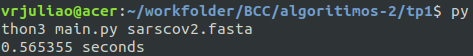
\includegraphics[scale=0.75]{Figuras/create-trie.png}
	\end{center}
	\caption{\label{fig:create-trie} Tempo de criação da árvore (processamento dos sufixos).}
\end{figure}

Na Figura \ref{fig:create-trie} apenas a linha que computa
\texttt{tree = sufix\_tree.SufixTree(text)} é considerada.
Da mesma forma computou-e o tempo de execução da obtenção da maior substring
que se repete na árvore apenas pelo tempo da chamada
\texttt(repetitions, indexes = tree.biggest\_substr()), e o tempo é obsevado
na Figura \ref{fig:biggest-substr}.

\begin{figure}[h]
	\begin{center}
		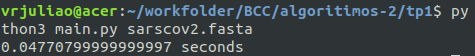
\includegraphics[scale=0.75]{Figuras/biggest-substr.png}
	\end{center}
	\caption{\label{fig:biggest-substr} Tempo para encontrar a maior substring que se repete na árvore.}
\end{figure}

Já o tempo total de execução foi obtido através considerando toda a função
\texttt{main}, incluindo o tempo de leitura da entrada e a impressão da resposta.
Dessa forma, a Figura \ref{fig:total-execution} demonstra a resposta que a
solução dá para o arquivo \texttt{sarscov2.fasta}.
A primeira linha representa a quantidade de repetições encontradas, a próxima
linha mostra a substring que se repete.
Por fim, a ultima linha impressa é referente ao tempo de execução de toda a
função principal.

\begin{figure}[h]
	\begin{center}
		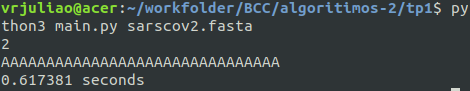
\includegraphics[scale=0.75]{Figuras/total-execution.png}
	\end{center}
	\caption{\label{fig:total-execution} Tempo total de execução.}
\end{figure}


A resposta obtida pelo Valgrind é demonstrada na Figura \ref{fig:valgrind}, que
demonstra uma alocação total de $7.936.935$ bytes.
O comando executado para a obtenção dessa resposta foi:
\lstset{language=bash}
\begin{lstlisting}[frame=single]
$ valgrind --tool=memcheck python3 -E -tt main.py sarscov2.fasta
\end{lstlisting}

\begin{figure}[h]
	\begin{center}
		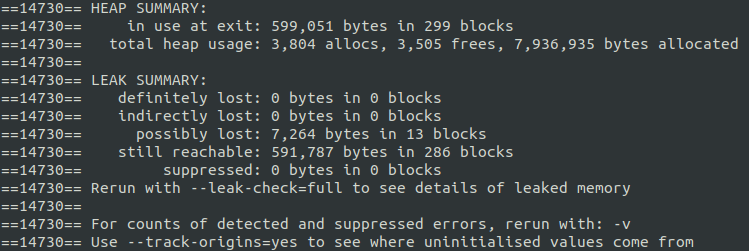
\includegraphics[scale=0.5]{Figuras/valgrind.png}
	\end{center}
	\caption{\label{fig:valgrind} Execução do Valgrind para obtenção da memória utilizada.}
\end{figure}